\documentclass{beamer}
%
% Choose how your presentation looks.
%
% For more themes, color themes and font themes, see:
% http://deic.uab.es/~iblanes/beamer_gallery/index_by_theme.html
%
\mode<presentation>
{
  \usetheme{Madrid}      % or try Darmstadt, Madrid, Warsaw, ...
  \usecolortheme{seahorse} % or try albatross, beaver, crane, ...
  \usefonttheme{serif}  % or try serif, structurebold, ...
  \setbeamertemplate{navigation symbols}{}
  \setbeamertemplate{caption}[numbered]
} 

\usepackage[english]{babel}
\usepackage{kotex}
\usepackage{tikz}
\usepackage{listings}
\usepackage{pgffor}
\input{algorithmbisEnv.tex}

\title[3D 그래픽스 프로그래밍]{그래픽스 강의노트 05 - OpenGL 카메라}
\author{강영민}
\institute{동명대학교}
\date{2015년 6학기}

\begin{document}

%%%%%%%%%%%%%%%%%%%%%%%%%%%%%%%%%%%%%%%%%%%%%%%%%%%%%%%%%
\begin{frame}
  \titlepage
\end{frame}

% Uncomment these lines for an automatically generated outline.
%\begin{frame}{Outline}
%  \tableofcontents
%\end{frame}


%%%%%%%%%%%%%%%%%%%%%%%%%%%%%%%%%%%%%%%%%%%%%%%%%%%%%%%%%%
%\begin{frame}[fragile]{깊이 버퍼와 이중 버퍼 사용 예제}
%   \lstset{language=C++,frame=none,escapechar=^}%
%    \foreach \n in {1,26,...,50} {%
%       \only<+>{%
%            \edef\m{\the\numexpr\n+24\relax}%
%            \edef\thesubtitle{{Lines \n--\m\ / 50}}%
%            \expandafter\framesubtitle\thesubtitle
%            \lstinputlisting[firstline=\n,lastline=\m]{./Codes/L03_depthAndDoubleBuffers.tex}%
%       }%
%    }
%\end{frame}
%%%%%%%%%%%%%%%%%%%%%%%%%%%%%%%%%%%%%%%%%%%%%%%%%%%%%%%%%%

%%%%%%%%%%%%%%%%%%%%%%%%%%%%%%%%%%%%%%%%%%%%%%%%%%%%%%%%%
%\begin{frame}[fragile]{간단한 OpenGL 프로그램 테스트}
%\lstset{language=C++,escapechar=^} 
%\begin{lstlisting}
%#include "headers.h"
%
%void myDisplay() {
%   glClear(GL_COLOR_BUFFER_BIT);
%    glFlush();    
%}
%\end{lstlisting}
%\end{frame}
%%%%%%%%%%%%%%%%%%%%%%%%%%%%%%%%%%%%%%%%%%%%%%%%%%%%%%%%%%


%%%%%%%%%%%%%%%%%%%%%%%%%%%%%%%%%%%%%%%%%%%%%%%%%%%%%%%%%
\begin{frame}{카메라 좌표 1/2}

\begin{itemize}
\item 3차원 그래픽스에서 모든 정점은 카메라를 기준으로 좌표가 재배치
\item OpenGL에서 이 카메라 좌표계의 원점은 카메라의 위치가 되고, 카메라가 바라보는 방향이 $z$축의 음의 방향
\end{itemize}

\begin{figure}
    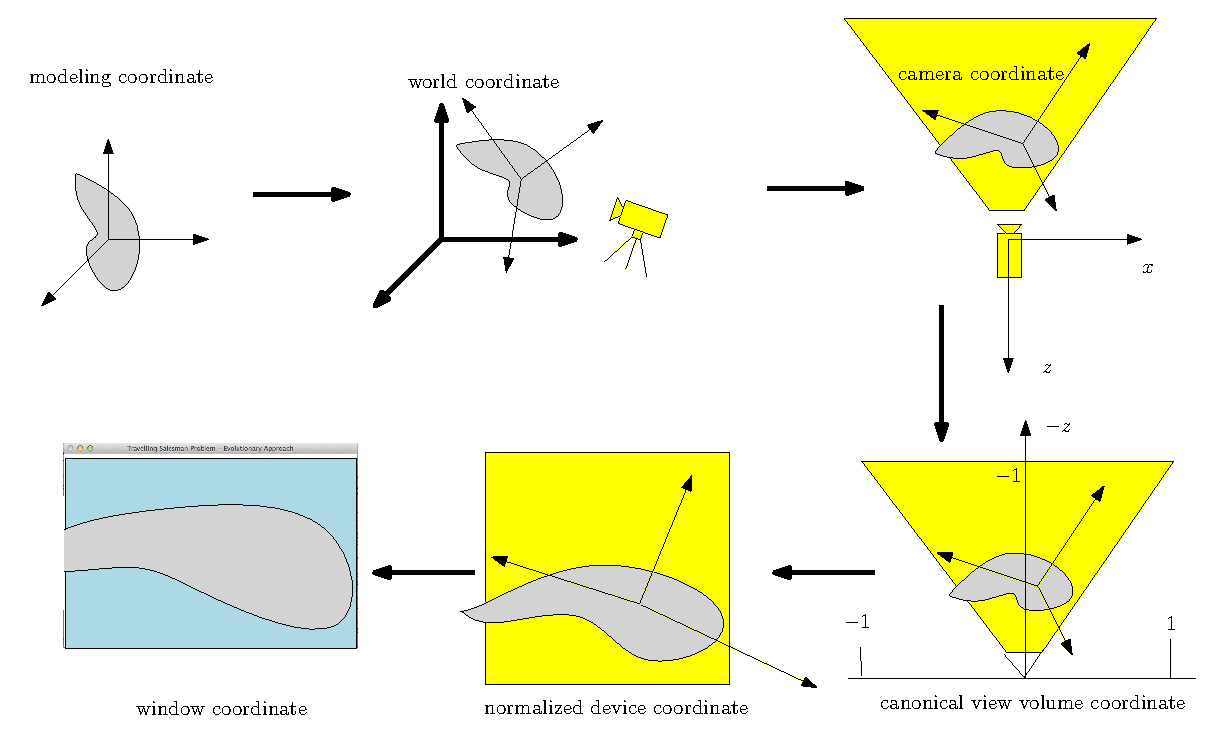
\includegraphics[height=6cm]{OGL_camera/coordinatesInPipeline.eps}
\end{figure}

\end{frame}
%%%%%%%%%%%%%%%%%%%%%%%%%%%%%%%%%%%%%%%%%%%%%%%%%%%%%%%%%

%%%%%%%%%%%%%%%%%%%%%%%%%%%%%%%%%%%%%%%%%%%%%%%%%%%%%%%%%
\begin{frame}{카메라 좌표 2/2}

\begin{itemize}
\item 모델링 좌표계를 기준으로 객체를 구성하는 각 정점의 좌표 결정
\item 객체에 적용되는 각종 변환들에 의해 전역 좌표(world coodinate)가 결정
\item 렌더링 파이프라인은 이를 화면에 출력하기 위해 카메라 좌표계로 변경
	\begin{itemize}
	\item 카메라의 위치가 원점이 되고, 카메라는 $z$축 음의 방향을 향함
	\end{itemize}
\item 관측볼륨의 변환
	\begin{itemize}
	\item 관측 볼륨 밖은 처리에서 제외
	\item 관측 볼륨은 클리핑 등이 효율적으로 이루어질 수 있는 표준 관측 볼륨(canonical viewing volume)으로 변환
	\item 표준 관측 볼륨은 정규 장치 좌표계로 변경: $x, y, z$의 범위가 모두 $[-1,1]$인 정육면체 공간
	\end{itemize}
\item 투영: 정규 장치 좌표에서 $z$ 값을 버리고 $(x,y)$만 취함
\end{itemize}

\end{frame}
%%%%%%%%%%%%%%%%%%%%%%%%%%%%%%%%%%%%%%%%%%%%%%%%%%%%%%%%%



%%%%%%%%%%%%%%%%%%%%%%%%%%%%%%%%%%%%%%%%%%%%%%%%%%%%%%%%%
\begin{frame}{직교 투영 카메라 1/4}

{\small
\begin{itemize}
\item 디폴트 카메라의 경우 중심이 원점이고, 각 변의 길이가 2인 상자 모양인데, 이 위치와 길이를 변경할 수 있다. 이를 지원하는 함수는 {\sf glOrtho}
\item glOrtho(float left, float right, float bottom, float top, float near, float far);
\end{itemize}
}

\begin{figure}
    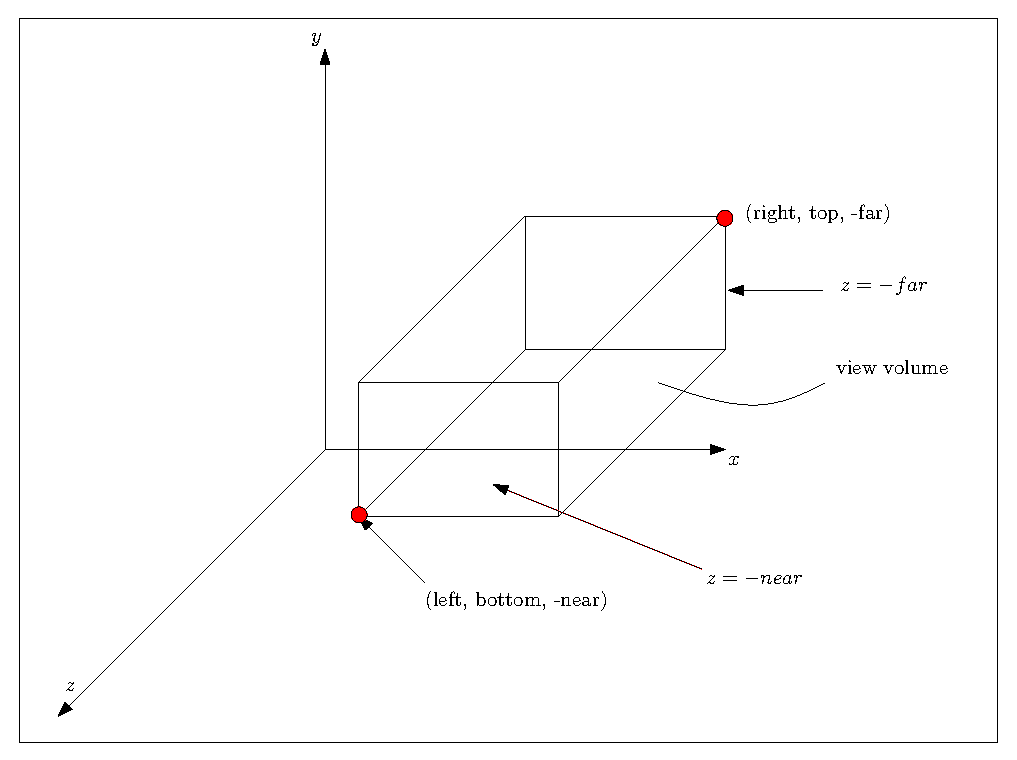
\includegraphics[height=5cm]{OGL_camera/cameraViewVolume.eps}
\end{figure}

\end{frame}
%%%%%%%%%%%%%%%%%%%%%%%%%%%%%%%%%%%%%%%%%%%%%%%%%%%%%%%%%

%%%%%%%%%%%%%%%%%%%%%%%%%%%%%%%%%%%%%%%%%%%%%%%%%%%%%%%%%
\begin{frame}[fragile]{직교 투영 카메라 2/4}

\begin{itemize}
\item OpenGL은 관측공간(view volume)을 최초의 디폴트 카메라 공간으로 옮기는 변환을 수행
\item 관측공간 내부의 모든 객체가 디폴트 관측 공간인 (-1,1)$\times$(-1,1)$\times$(-1,1)로 옮겨지도록 하는 것
	\begin{itemize}
	\item ‘정규 관측 공간(canonical view volume)‘
	\end{itemize}
\item $x$ 축으로는 범위 $[left, right]$를 $[-1, 1]$로 변경하는 것
\end{itemize}

\begin{eqnarray}
x' = \left ( \frac{2}{right-left} \right ) x - \frac{right+left}{right-left} \nonumber
\end{eqnarray}

\end{frame}
%%%%%%%%%%%%%%%%%%%%%%%%%%%%%%%%%%%%%%%%%%%%%%%%%%%%%%%%%

%%%%%%%%%%%%%%%%%%%%%%%%%%%%%%%%%%%%%%%%%%%%%%%%%%%%%%%%%
\begin{frame}[fragile]{직교 투영 카메라 3/4}

\begin{eqnarray}
x' = \left ( \frac{2}{right-left} \right ) x - \frac{right+left}{right-left} \nonumber
\end{eqnarray}

\begin{figure}[h!]
  \centering
    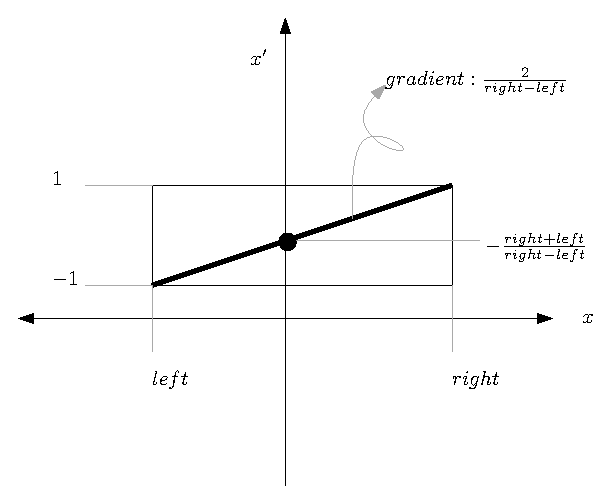
\includegraphics[height=6cm]{OGL_camera/glOrthoXProjection.eps}
    \caption{glOrtho 투영에 의한 $x$ 좌표의 변경}
    \label{fig:OGL_camera:glOrthoXProjection}
\end{figure}

\end{frame}
%%%%%%%%%%%%%%%%%%%%%%%%%%%%%%%%%%%%%%%%%%%%%%%%%%%%%%%%%

%%%%%%%%%%%%%%%%%%%%%%%%%%%%%%%%%%%%%%%%%%%%%%%%%%%%%%%%%
\begin{frame}[fragile]{직교 투영 카메라 4/4}

비슷한 방법으로 $y$ 축 좌표의 변경도 가능하다.

\begin{eqnarray}
y' = \left ( \frac{2}{top-bottom} \right ) y - \frac{top+bottom}{top-bottom} \nonumber
\end{eqnarray}

$z$ 축 좌표는 부호가 바꾸어 적용

\begin{eqnarray}
z' = - \left ( \frac{2}{far-near} \right ) z - \frac{far+near}{far-near} \nonumber
\end{eqnarray}

glOrtho에 의해 결정되는 투영행렬 
\begin{eqnarray}
\left ( 
\begin{array}{cccc} \nonumber
\frac{2}{right-left}& 0 & 0 & - \frac{right+left}{right-left}\\ \nonumber
0& \frac{2}{top-bottom} & 0 & - \frac{top+bottom}{top-bottom}\\ \nonumber
0& 0 & \frac{2}{far-near} & - \frac{far+near}{far-near}\\ \nonumber
0& 0 & 0 & 1 \nonumber
\end{array} 
\right )
\end{eqnarray}

\end{frame}
%%%%%%%%%%%%%%%%%%%%%%%%%%%%%%%%%%%%%%%%%%%%%%%%%%%%%%%%%


%%%%%%%%%%%%%%%%%%%%%%%%%%%%%%%%%%%%%%%%%%%%%%%%%%%%%%%%%
\begin{frame}[fragile]{원근 투영 카메라}

\begin{itemize}
\item 실제 카메라나 우리 눈
	\begin{itemize}
	\item멀리 있는 것은 작게 보이고 가까이 있는 것은 크게 보임
	\item 빛이 관측 지점으로 모이면서 형성되는 선을 따라 원근투영되기 때문
	\end{itemize}
\item 이러한 원근 투영을 설정하는 방법은 {\sf glFrustum}과 {\sf gluPerspective}
\end{itemize}

\begin{figure}[h!]
  \centering
    \includegraphics[height=6cm]{OGL_camera/perspectiveCam.eps}
\end{figure}

\end{frame}
%%%%%%%%%%%%%%%%%%%%%%%%%%%%%%%%%%%%%%%%%%%%%%%%%%%%%%%%%

%%%%%%%%%%%%%%%%%%%%%%%%%%%%%%%%%%%%%%%%%%%%%%%%%%%%%%%%%
\begin{frame}[fragile]{원근 투영 카메라}

\begin{itemize}
\item 실제 카메라나 우리 눈
	\begin{itemize}
	\item멀리 있는 것은 작게 보이고 가까이 있는 것은 크게 보임
	\item 빛이 관측 지점으로 모이면서 형성되는 선을 따라 원근투영되기 때문
	\end{itemize}
\item 이러한 원근 투영을 설정하는 방법은 {\sf glFrustum}과 {\sf gluPerspective}
\end{itemize}

\begin{figure}[h!]
  \centering
    \includegraphics[height=6cm]{OGL_camera/perspectiveCam.eps}
\end{figure}

\end{frame}
%%%%%%%%%%%%%%%%%%%%%%%%%%%%%%%%%%%%%%%%%%%%%%%%%%%%%%%%%

%%%%%%%%%%%%%%%%%%%%%%%%%%%%%%%%%%%%%%%%%%%%%%%%%%%%%%%%%
\begin{frame}[fragile]{직교 투영과 원근 투영 비교}

\begin{figure}[h!]
  \centering
    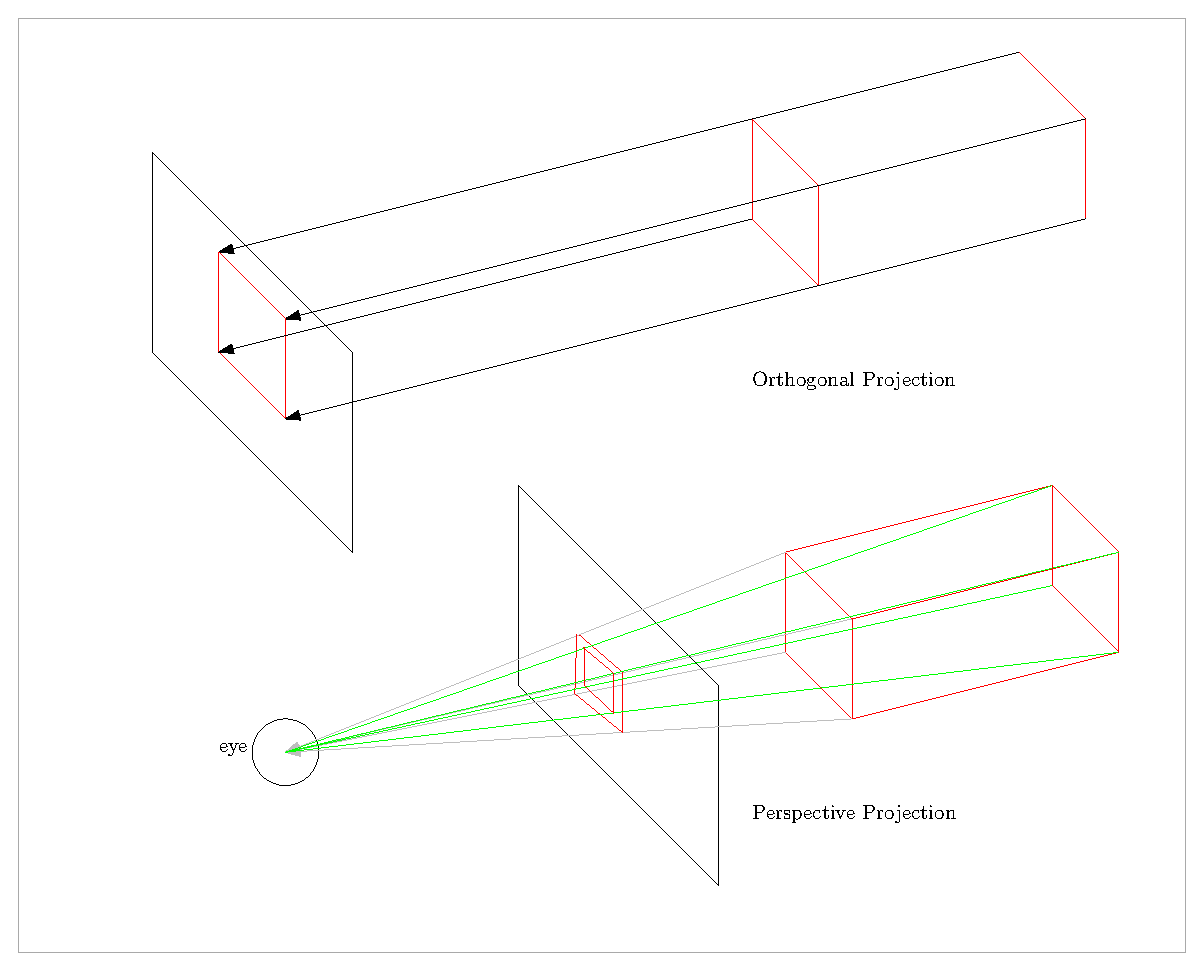
\includegraphics[height=7cm]{OGL_camera/projection.eps}
\end{figure}

\end{frame}
%%%%%%%%%%%%%%%%%%%%%%%%%%%%%%%%%%%%%%%%%%%%%%%%%%%%%%%%%

%%%%%%%%%%%%%%%%%%%%%%%%%%%%%%%%%%%%%%%%%%%%%%%%%%%%%%%%%
\begin{frame}[fragile]{절두체 공간}

\begin{itemize}
\item 3차원 그래픽스의 표준적인 카메라 모델은 렌더링의 대상이 되는 영역을 일정한 범위로 제한
\item 원근이 있는 투영의 경우에는 절두체(frustum) 모양을 이룬다.
\end{itemize}

\begin{figure}[h!]
  \centering
    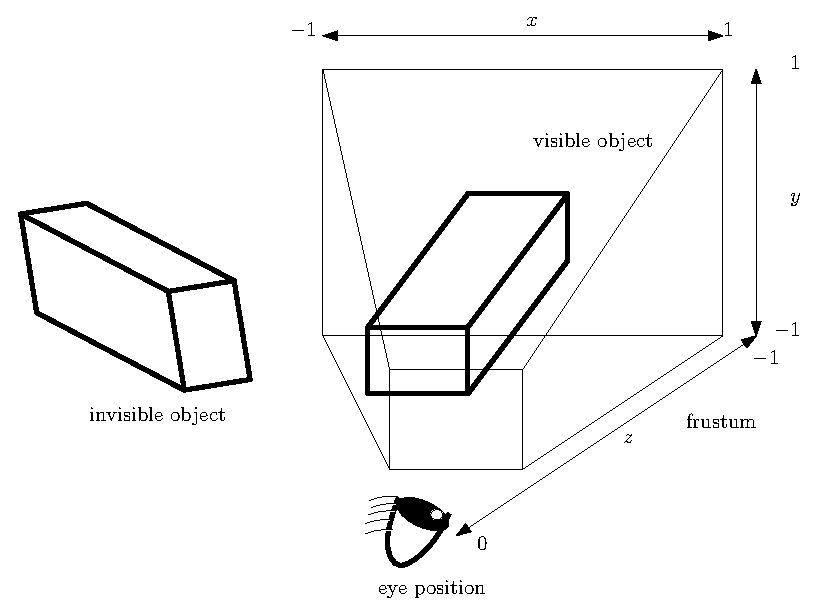
\includegraphics[height=6cm]{OGL_camera/frustumConcept.eps}
\end{figure}

\end{frame}
%%%%%%%%%%%%%%%%%%%%%%%%%%%%%%%%%%%%%%%%%%%%%%%%%%%%%%%%%

%%%%%%%%%%%%%%%%%%%%%%%%%%%%%%%%%%%%%%%%%%%%%%%%%%%%%%%%%
\begin{frame}[fragile]{정규 장치 좌표계}

화면에 출력을 하기 위해서는 관측 볼륨을 정규 장치 좌표계로 바꾼다.

\begin{figure}[h!]
  \centering
    \includegraphics[height=7cm]{OGL_camera/deviceCoordinate.eps}
\end{figure}

\end{frame}
%%%%%%%%%%%%%%%%%%%%%%%%%%%%%%%%%%%%%%%%%%%%%%%%%%%%%%%%%

%%%%%%%%%%%%%%%%%%%%%%%%%%%%%%%%%%%%%%%%%%%%%%%%%%%%%%%%%
\begin{frame}[fragile]{카메라의 위치변경}

\begin{itemize}
\item {\sf gluPerspective}를 사용하여도 카메라는 여전히 원점 (0,0,0)에 놓임
\item 카메라를 원하는 곳으로 옮겨주는 함수: {\sf gluLookAt}
\end{itemize}

{\tiny gluLookAt(float $eye_x$, float $eye_y$, float $eye_z$,  float $at_x$, float $at_y$, float $at_z$,  float $up_x$, float $up_y$, float $up_z$)}

\begin{figure}[h!]
  \centering
    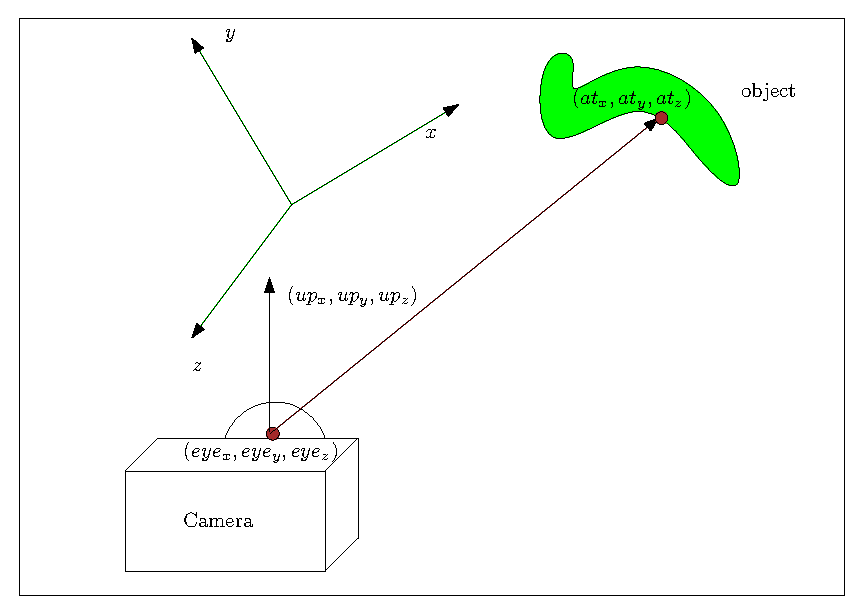
\includegraphics[height=6cm]{OGL_camera/cameraPositioning.eps}
\end{figure}

\end{frame}
%%%%%%%%%%%%%%%%%%%%%%%%%%%%%%%%%%%%%%%%%%%%%%%%%%%%%%%%%

%%%%%%%%%%%%%%%%%%%%%%%%%%%%%%%%%%%%%%%%%%%%%%%%%%%%%%%%%
\begin{frame}[fragile]{행렬모드(Matrix mode)}

{\small
\begin{itemize}
\item OpenGL은 세 종류의 행렬 모드: 텍스처 행렬, 모델뷰 행렬, 투영행렬
\item 가상공간 내의 좌표를 결정하는 행렬은 모델뷰 행렬과 투영행렬
\item 모델뷰행렬(modelview matrix)은 공간 내에서 가상 객체를 변환하여 좌표를 변경하는 데에 사용
\item 투영행렬(projection matrix)은 가상 객체를 투영면에 옮겨 놓는 데에 사용
\item {\sf gluPerspective} 함수는 투영의 특성을 변경하는 것이므로 투영행렬 모드
\item {\sf gluLookAt}은 투영의 특성이 아니라 카메라의 위치를 옮기는 것이고, 이는 바꾸어 말해 물체의 위치를 카메라 기준에서 옮기는 것이므로 모델뷰 행렬을 변경
\end{itemize}


\begin{verbatim}
glMatrixMode(GL_PROJECTION);
glLoadIdentity();
gluPerspective(60, 1.0, 0.1, 100.0);
glMatrixMode(GL_MODELVIEW);
glLoadIdentity();
gluLookAt(1.0,1.0,1.0, 0.0, 0.0, 0.0, 0.0, 1.0, 0.0);
\end{verbatim}
}

\end{frame}
%%%%%%%%%%%%%%%%%%%%%%%%%%%%%%%%%%%%%%%%%%%%%%%%%%%%%%%%%

%%%%%%%%%%%%%%%%%%%%%%%%%%%%%%%%%%%%%%%%%%%%%%%%%%%%%%%%%
\begin{frame}[fragile]{glFrustum}

{\small 
카메라의 원근 투영을 설정하는 가장 기본적인 방법은 {\sf glFrustum} 함수를 이용

glFrustum(float left, float right, float bottom, float top, float near, float far);
}

\begin{figure}[h!]
  \centering
    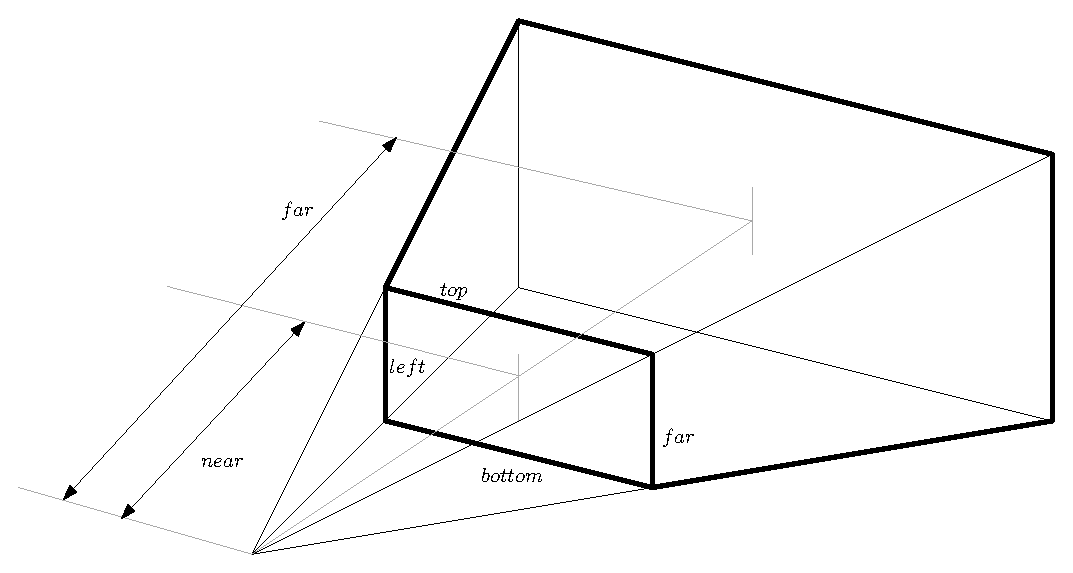
\includegraphics[height=6cm]{OGL_camera/glFrustum.eps}
\end{figure}
\end{frame}
%%%%%%%%%%%%%%%%%%%%%%%%%%%%%%%%%%%%%%%%%%%%%%%%%%%%%%%%%

%%%%%%%%%%%%%%%%%%%%%%%%%%%%%%%%%%%%%%%%%%%%%%%%%%%%%%%%%
\begin{frame}[fragile]{glFrustum}

glFrustum 공간을 평행 투영 공간으로 바꾸기 위한 변환

\begin{eqnarray}
\label{eq:OGL_camera:glFrustumMatrix}
\left ( 
\begin{array}{cccc} \nonumber
\frac{2 near}{right-left}& 0 & \frac{right+left}{right - left} & 0\\ \nonumber
0& \frac{2 near}{top-bottom} & \frac{top+bottom}{top - bottom} & 0\\ \nonumber
0& 0 & -\frac{far+near}{far-near} & \frac{-2 near \cdot far}{far-near}\\ \nonumber
0& 0 & -1 & 0 \nonumber
\end{array} 
\right )
\end{eqnarray}

\end{frame}
%%%%%%%%%%%%%%%%%%%%%%%%%%%%%%%%%%%%%%%%%%%%%%%%%%%%%%%%%

%%%%%%%%%%%%%%%%%%%%%%%%%%%%%%%%%%%%%%%%%%%%%%%%%%%%%%%%%
\begin{frame}[fragile]{glFrustum}

glFrustum 공간을 평행 투영 공간으로 바꾸기 위한 변환

\begin{eqnarray}
\label{eq:OGL_camera:glFrustumMatrix}
\left ( 
\begin{array}{cccc} \nonumber
\frac{2 near}{right-left}& 0 & \frac{right+left}{right - left} & 0\\ \nonumber
0& \frac{2 near}{top-bottom} & \frac{top+bottom}{top - bottom} & 0\\ \nonumber
0& 0 & -\frac{far+near}{far-near} & \frac{-2 near \cdot far}{far-near}\\ \nonumber
0& 0 & -1 & 0 \nonumber
\end{array} 
\right )
\end{eqnarray}

\end{frame}
%%%%%%%%%%%%%%%%%%%%%%%%%%%%%%%%%%%%%%%%%%%%%%%%%%%%%%%%%


%%%%%%%%%%%%%%%%%%%%%%%%%%%%%%%%%%%%%%%%%%%%%%%%%%%%%%%%%
\begin{frame}[fragile]{glFrustum 투영 유도}

{\small
\begin{itemize}
\item 볼륨 안의 $\mathbf p$가 가까운 쪽 클리핑 평면 $z=-near$에 떨어진 좌표 구하기
\end{itemize}

\begin{figure}[h!]
  \centering
    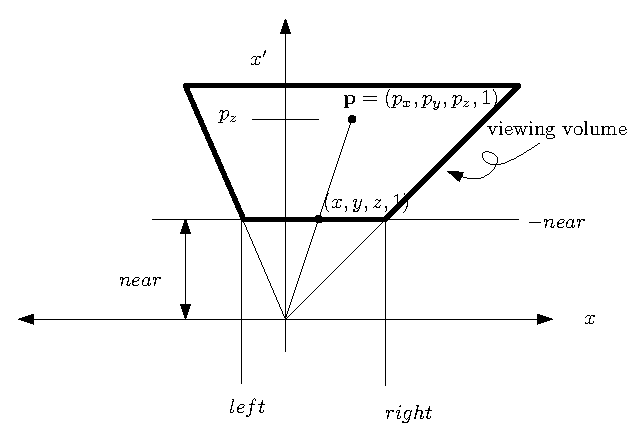
\includegraphics[height=5cm]{OGL_camera/glFrustumXProjection.eps}
\end{figure}

$p_x:p_z = x:-near$임을 알 수 있고, 다음과 같은 식을 유도할 수 있다.

\begin{eqnarray}
x = - near \frac{p_x}{p_z}
\end{eqnarray}
}

\end{frame}
%%%%%%%%%%%%%%%%%%%%%%%%%%%%%%%%%%%%%%%%%%%%%%%%%%%%%%%%%

%%%%%%%%%%%%%%%%%%%%%%%%%%%%%%%%%%%%%%%%%%%%%%%%%%%%%%%%%
\begin{frame}[fragile]{glFrustum 투영 유도}

이렇게 해서 얻는 $x$ 좌표를 직교 투영에서 살펴본 바와 같이
정규 장치 좌표계, 즉 $[-1,1]$의 범위로 옮김

\begin{eqnarray}
x' = \left ( - \frac{2 near}{right-left} \right ) \frac{p_x}{p_z} - \frac{right+left}{right-left} ] \nonumber
\end{eqnarray}


\end{frame}
%%%%%%%%%%%%%%%%%%%%%%%%%%%%%%%%%%%%%%%%%%%%%%%%%%%%%%%%%


%%%%%%%%%%%%%%%%%%%%%%%%%%%%%%%%%%%%%%%%%%%%%%%%%%%%%%%%%
\begin{frame}[fragile]{glFrustum 투영 유도}

비슷한 방법으로 $y$ 좌표를 구하고 이를 정규 장치 좌표계의 좌표 $y'$로 바꾸는 작업

\begin{eqnarray}
\label{eq:OGL_camera:frustumYProjection}
y' = \left ( - \frac{2 near}{top-bottom} \right ) \frac{p_y}{p_z} - \frac{top + bottom}{top - bottom}
\end{eqnarray}


\end{frame}
%%%%%%%%%%%%%%%%%%%%%%%%%%%%%%%%%%%%%%%%%%%%%%%%%%%%%%%%%

%%%%%%%%%%%%%%%%%%%%%%%%%%%%%%%%%%%%%%%%%%%%%%%%%%%%%%%%%
\begin{frame}[fragile]{glFrustum 투영 유도}

$x$와 $y$의 투영과 같은 꼴로 표현

$$z' = \frac{\alpha}{p_z} + \beta$$

[$near$, $far$]를 [-1,1]로

\begin{eqnarray}
-1 & = & \frac{\alpha}{near} + \beta \\ \nonumber
  1 & = & \frac{\alpha}{far} + \beta
\end{eqnarray}

이 이원일차연립방정식을 풀면 $\alpha$와 $\beta$를 다음과 같이 구할 수 있다.

$$\alpha = \frac{near \cdot far}{far - near}, ~~~ \beta = \frac{far+near}{far-near}$$


\end{frame}
%%%%%%%%%%%%%%%%%%%%%%%%%%%%%%%%%%%%%%%%%%%%%%%%%%%%%%%%%

%%%%%%%%%%%%%%%%%%%%%%%%%%%%%%%%%%%%%%%%%%%%%%%%%%%%%%%%%
\begin{frame}[fragile]{glFrustum 투영 유도}

\begin{eqnarray}
\left (
\begin{array}{c}
x\\
y\\
z\\
1
\end{array} 
\right ) =
\left ( 
\begin{array}{c}
-x \cdot p_x\\
-y \cdot p_y\\
-z \cdot p_z\\
-p_z
\end{array} 
\right )=
\left ( 
\begin{array}{cccc}
\frac{2 near}{right - left} p_x + \frac{right+left}{right-left} p_z \\
\frac{2 near}{top - bottom} p_y + \frac{top+bottom}{top-bottom} p_z \\
-\frac{far + near}{right - left} p_z - \frac{2 near \cdot far}{far - near} \\
- p_z \\ \nonumber
\end{array}
\right )
\end{eqnarray}

이상의 결과를 통해 우리는 {\sf glFrustum}에 의해 만들어지는 투영행렬이 
식 \ref{eq:OGL_camera:glFrustumMatrix}과 같음을 알 수 있다.
여기서 {\sf far}의 값이 무한대인 경우, 즉, 먼쪽 클리핑 평면이 없는 경우의 투영행렬이 어떻게 될지 고민해 보라.


\end{frame}
%%%%%%%%%%%%%%%%%%%%%%%%%%%%%%%%%%%%%%%%%%%%%%%%%%%%%%%%%

%%%%%%%%%%%%%%%%%%%%%%%%%%%%%%%%%%%%%%%%%%%%%%%%%%%%%%%%%
\begin{frame}[fragile]{glFrustum과 gluPerspective}

\begin{verbatim}
gluPerspective(fovy, aspect, near, far);
glFrustum(left,right,bottom,top,near,far);
\end{verbatim}

$$top = near \cdot \tan \frac{\theta}{2}$$
$$bottom = -near \cdot \tan \frac{\theta}{2}$$
$$right = top \cdot aspect$$
$$left = bottom \cdot aspect$$


\end{frame}
%%%%%%%%%%%%%%%%%%%%%%%%%%%%%%%%%%%%%%%%%%%%%%%%%%%%%%%%%

\end{document}












%%%%%%%%%%%%%%%%%%


우리는 앞서 직관적 이해가 쉬운 gluPerspective를 사용하였다. 그러나 내부적으로 이 함수는 glFrustum을 호출하게 되어 있다. gluPerspective에 사용된 파라미터를 이용하여 glFrustum 함수에 적용되는 파라미터를 계산할 수 있는데, 이 둘은 다음 관계를 갖는다.



\section{오픈지엘(OpenGL) 카메라의 특성 제어}\index{카메라!오픈지엘 카메라}\index{OpenGL!camera}

이제 지금까지 사용한 간단한 카메라를 조금 더 유용하게 개선하여 보자. 우선 지금까지의 카메라는 다음과 같은 심각한 문제를 가지고 있다.
카메라의 종횡비가 1이어서 창의 크기를 변경하면 그려지는 결과에 왜곡이 발생한다. 즉 그림 \ref{fig:OGL_camera:aspectRatioDistort}과 같이 정사각형 창의 경우에는 제대로 그려지지만, 상하로 긴 창에서는 주전자도 함께 길어진다. 창이 좌우로 길어져도 비슷한 왜곡이 발생한다.

\begin{figure}[h!]
  \centering
    \fbox{\includegraphics[height=4cm]{OGL_camera/aspectRatioDistort.png}}
    \caption{종횡비(aspect ratio)에 따라 왜곡되는 화면}
    \label{fig:OGL_camera:aspectRatioDistort}
\end{figure}

창 크기가 변경되는 이벤트의 처리 함수는 GLUT의 API를 이용하여 {\sf glutReshapeFunc} 함수로 등록할 수 있다. 이때 등록되는 콜백(callback) 함수는 다음의 프로토타입(prototype)을 갖는다.

\begin{verbatim}
void reshapeFunction(int w, int h);
\end{verbatim}

여기에서 {\sf w}와 {\sf h}는 새롭게 변경된 창의 가로와 세로 픽셀 수이다. 이를 이용하여 코드 \ref{code:OGL_camera:reshapeWindow}과 같이 
{\sf glOrtho}를 설정하면 그림 \ref{fig:OGL_camera:aspectRatioNoDistort}에서 확인할 수 있는 바와 같이 왜곡없는 카메라를 구현할 수 있다.



\begin{algorithmbis}[창 크기 변경에 따른 카메라 재설정]\label{code:OGL_camera:reshapeWindow}
\lstset{language=C++, escapechar=^} 
\begin{lstlisting}
^{\sf [[헤더 파일 포함하기]]^

void init(int argc, char **argv) {
   ^{\sf [[윈도우, 버퍼 초기화 작업]]^

   glMatrixMode(GL_PROJECTION);
   glLoadIdentity();
   glOrtho(-2.0, 2.0, -2.0, 2.0, -2.0, 2.0);
}
void reshape(int w, int h) {
   float asp = float(w)/float(h);
   glViewport(0, 0, w, h);
   glMatrixMode(GL_PROJECTION);
   glLoadIdentity();
   glOrtho(-2.0*asp, 2.0*asp,    -2.0, 2.0,  -2.0, 2.0);
   glutPostRedisplay();
}
void display() {
   glClear(GL_COLOR_BUFFER_BIT);
   glMatrixMode(GL_MODELVIEW);
   glLoadIdentity();
   glutWireTeapot(1.0);
   glutSwapBuffers();
}
int main(int argc, char **argv) {
   init(argc, argv);
   glutDisplayFunc(display);
   glutReshapeFunc(reshape);
   glutMainLoop();
}
\end{lstlisting}
\end{algorithmbis}


\begin{figure}[h!]
  \centering
    \fbox{\includegraphics[height=4cm]{OGL_camera/aspectRatioNoDistort.png}}
    \caption{종횡비(aspect ratio)가 달라도 왜곡되지 않는 화면}
    \label{fig:OGL_camera:aspectRatioNoDistort}
\end{figure}

{\sf gluPerspective}를 사용할 경우에는 더욱 간단하다. 이 함수의 두 번째 파라미터로 종횡비를 바로 입력하면 된다. 그러면 {\sf gluPerspective}는 
적절한 {\sf glFrustum}을 계산한다.
키보드 이벤트를 이용하여 카메라를 직교 카메라(orthographic camera)와 원근 카메라(perspective camera)로 변경할 수 있도록 할 것이며, 
카메라의 줌인(zoom-in), 줌아웃(zoom-out)도 가능하게 할 것이다.
우선 키보드를 처리하는 콜백함수의 등록을 한다. 이는 {\sf glutKeyboardFunc} 함수를 통해 가능하다. 
카메라의 종류는 {\sf bOrthoCam}이 결정한다. 이 값이 {\sf true}이면 
{\sf glOrtho}를 불러 직교 투영 카메라를 사용하고, {\sf false}이면 {\sf gluPerspective}를 불러 원근 투영 카메라를 사용한다. 
다음으로 줌인/줌아웃은 {\sf zoomFactor}라는 변수에 의해 결정된다. 이 값이 커지면 줌인, 작아지면 줌아웃이 되도록 할 것이다. 
이를 구현하기 위해서 {\sf glOrtho}와 {\sf glPerspective}에 실제로 적용하는 방식은 약간 다르다.

{\sf glOrtho}의 경우 줌인/줌아웃을 수행하기 위해서는 좌우, 상하의 값을 변경해야 한다. 이는 {\sf zoomFactor}로 이 값들을 나눠주면 된다. 

\begin{verbatim}
glOrtho(-2.0*aspRatio/zoomFactor, 2.0*aspRatio/zoomFactor, 
        -2.0/zoomFactor, 2.0/zoomFactor, 
        -200.0, 200.0);
\end{verbatim}


{\sf gluPerspective}는 첫 번째 파라미터가 시야각을 결정한다. 줌인이라는 것은 망원렌즈의 배율이 올라가는 것과 같고, 이는 투영의 각을 좁히는 것으로 흉내낼 수 있다. 따라서 {\sf zoomFactor}를 이용하여 이 {\sf fovy}, 즉 시야각을 나눠주면 된다.

\begin{verbatim}
gluPerspective(60/zoomFactor, aspRatio, 0.1, 100);
\end{verbatim}

또한 {\sf glOrtho}를 사용할 때에는 카메라가 원점에 있었도 문제가 없지만, {\sf gluPerspective}를 사용할 때에는 
카메라가 원점에 있으면 이 근처에 있는 주전자가 너무 크며, 일부 면을 볼 수 없다. 이를 해결하기 위해서는 카메라의 위치를 
{\sf gluLookAt}을 통해 관측가능한 곳으로 이동해 놓는다.
따라서 이 프로그램은 다음 코드 \ref{code:OGL_camera:cameraLensControl}과 같이 수정하여 ‘m’ 키에 의해 직교투영 카메라나 원근투영 카메라로 상호 변환될 수 있으며, ‘$<$‘ 키와 ‘$>$’를 이용하여 확대축소가 가능하다. 코드는 다음과 같이 정리된다.

\begin{algorithmbis}[카메라 렌즈 특성 선택 및 조작]\label{code:OGL_camera:cameraLensControl}
\lstset{language=C++, escapechar=^} 
\begin{lstlisting}
bool  bOrthoCam = true;
float aspRatio = 1.0;
float zoomFactor = 1.0;
void setCamera(void) {
   glMatrixMode(GL_PROJECTION);
   glLoadIdentity();
   if (bOrthoCam) {
      glOrtho(-2.0*aspRatio/zoomFactor, 
               2.0*aspRatio/zoomFactor, 
              -2.0/zoomFactor, 2.0/zoomFactor, 
              -200.0, 200.0);
   }
   else { // perspective camera
      gluPerspective(60/zoomFactor, aspRatio, 0.1, 100);
   }
}
void init(int argc, char **argv) {
   ^{\sf [[필요한 윈도우, 버퍼, 카메라 초기화 작업]]^
}
void keyboard(unsigned char k, int x, int y) {
   switch (k) {
      case 'm': bOrthoCam = bOrthoCam?false:true; break; // ^{\it 카메라 변경}^
      case '<': zoomFactor *= 0.95; break; // ^{\it 줌 아웃}^
      case '>': zoomFactor *= 1.05; break; // ^{\it 줌 인}^
      default: break;
   }
   setCamera();
   glutPostRedisplay();
}
void reshape(int w, int h) {
   aspRatio = float(w)/float(h);
   glViewport(0, 0, w, h);
   setCamera();
}
void display() {
   glClear(GL_COLOR_BUFFER_BIT);
   glMatrixMode(GL_MODELVIEW);
   glLoadIdentity();
   gluLookAt(0.0, 0.0, 3.0, 0.0, 0.0, 0.0, 0.0, 1.0, 0.0);
   glutWireTeapot(1.0);
   glutSwapBuffers();
}
int main(int argc, char **argv) {
   init(argc, argv);
   glutDisplayFunc(display);
   glutReshapeFunc(reshape);
   glutKeyboardFunc(keyboard);
   glutMainLoop();
}
\end{lstlisting}
\end{algorithmbis}

코드 \ref{code:OGL_camera:cameraLensControl}를 구현한 결과에서는 그림 \ref{fig:OGL_camera:cameraLensControl}와 같이 다양한 렌즈 특성을 테스트 할 수 있다.
\begin{figure}[h!]
  \centering
    \fbox{\includegraphics[height=4cm]{OGL_camera/cameraLensControl.png}}
    \caption{다양한 카메라 렌즈 특성을 설정한 결과}
    \label{fig:OGL_camera:cameraLensControl}
\end{figure}

카메라와 투영행렬에 대한 더 자세한 설명을 위해서는 \cite{lengyel2004mathematics,ryu20043d,dunn20113d} 등을 참고하라.

